\section{Technical foundations and historical method families}
\label{sec:methods}

PHASE-TTC grew through four model families: predictive embedding, geometry-constrained endpoint estimation, phase-domain temporal refinement, and RGB-anchored event fusion. Each family tests a different mechanism with its own objective and inference path. \evidence{M01--M14}

\begin{figure}[H]
\centering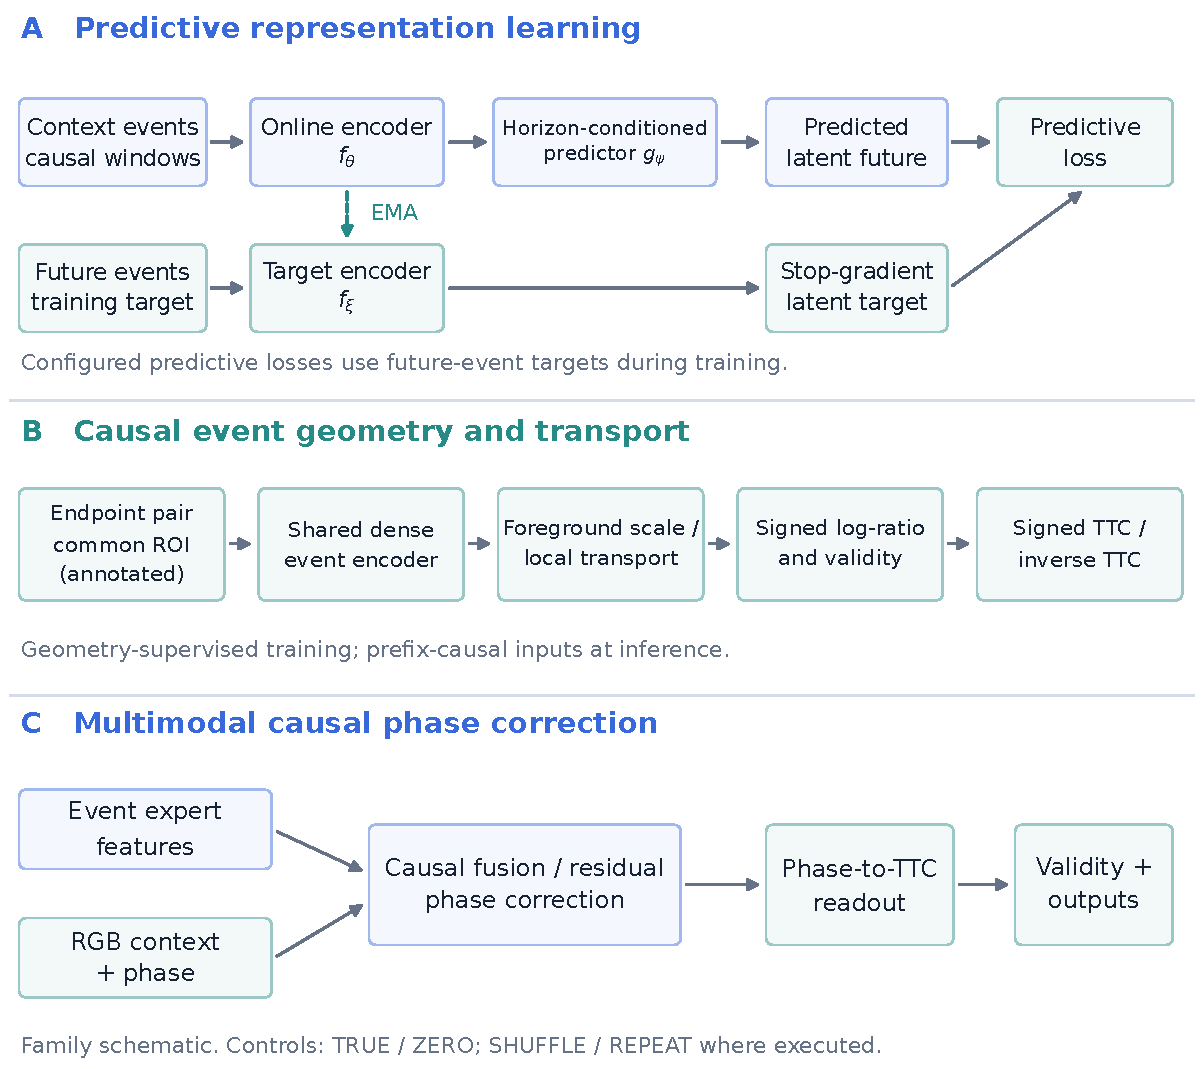
\includegraphics[width=\linewidth,height=.80\textheight,keepaspectratio]{figures/architecture.pdf}
\caption{\textbf{Selected model families.} (A) Predictive latent learning uses a training-only target branch. (B) Causal scale and transport map endpoint geometry to signed motion. (C) Phase-domain fusion combines event and RGB evidence. Panel A contains the JEPA objective; Sections~\ref{sec:phase-refinement} and~\ref{sec:train40} detail the later temporal and fusion paths.}
\label{fig:architecture}
\end{figure}
\FloatBarrier

\subsection{Events, temporal windows, and object coordinates}
An event stream is a sequence $\mathcal E=\{(x_i,y_i,t_i,p_i)\}_{i=1}^N$, with integer microsecond timestamps and normalized polarity $p_i\in\{-1,+1\}$. \texttt{EventBatch} stores aligned NumPy arrays for these fields. Each context window is anchored at its end time. Indexing rejects nonpositive durations, mismatched reference times, and future windows that begin before context ends. Causality tests cover crops, features, checkpoints, and calibration inputs. \evidence{M01}

The dense voxel representation distributes an event between adjacent temporal bins. For $K$ bins, duration $\Delta t$, and normalized time $u_i=(K-1)(t_i-t_0)/\Delta t$, the unnormalized representation is
\begin{equation}
 V_{p,k}(x,y)=\sum_i \mathbf 1[x_i=x,y_i=y,p_i=p]\max(0,1-|u_i-k|).
\end{equation}
Separate polarity yields $2K$ channels. Two flattened weighted histograms accumulate the adjacent-bin contributions without constructing a buffer with twice the event count. Optional robust scaling divides occupied voxels by the 95th percentile of their absolute magnitude; empty voxels remain zero. Median centering is omitted because equal occupied counts would collapse to zero. Event count, time surface, and sparse tokens remain separate representation alternatives. \evidence{M02}

Object-centred experiments use a common square region that covers both endpoint boxes, expands by a fixed margin, and maps both event windows into one raster coordinate system. Tight independent crops can erase apparent scale change. The resulting tensor is \emph{oracle-box-conditioned}: the event backbone assumes external localization even though its forward signature has no box argument. Causal-scale tests confirm that only the designated endpoint boxes affect the crop. \evidence{M03}

\begin{figure}[tbp]
\centering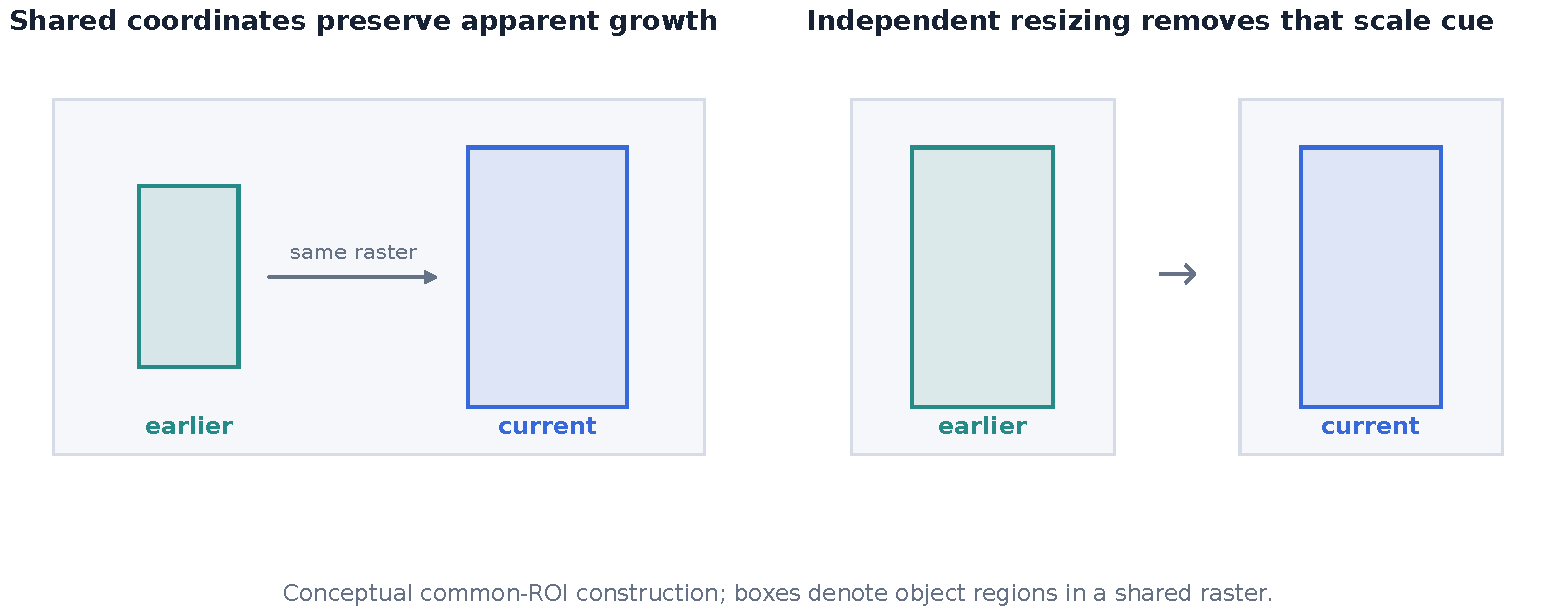
\includegraphics[width=\linewidth]{figures/crop_geometry.pdf}
\caption{\textbf{Shared coordinates preserve apparent expansion.} A common crop maps both endpoints at one spatial scale, whereas independent tight crops normalize away part of the size change. The diagram is schematic.}
\label{fig:crop}
\end{figure}

\begin{figure}[tbp]
\centering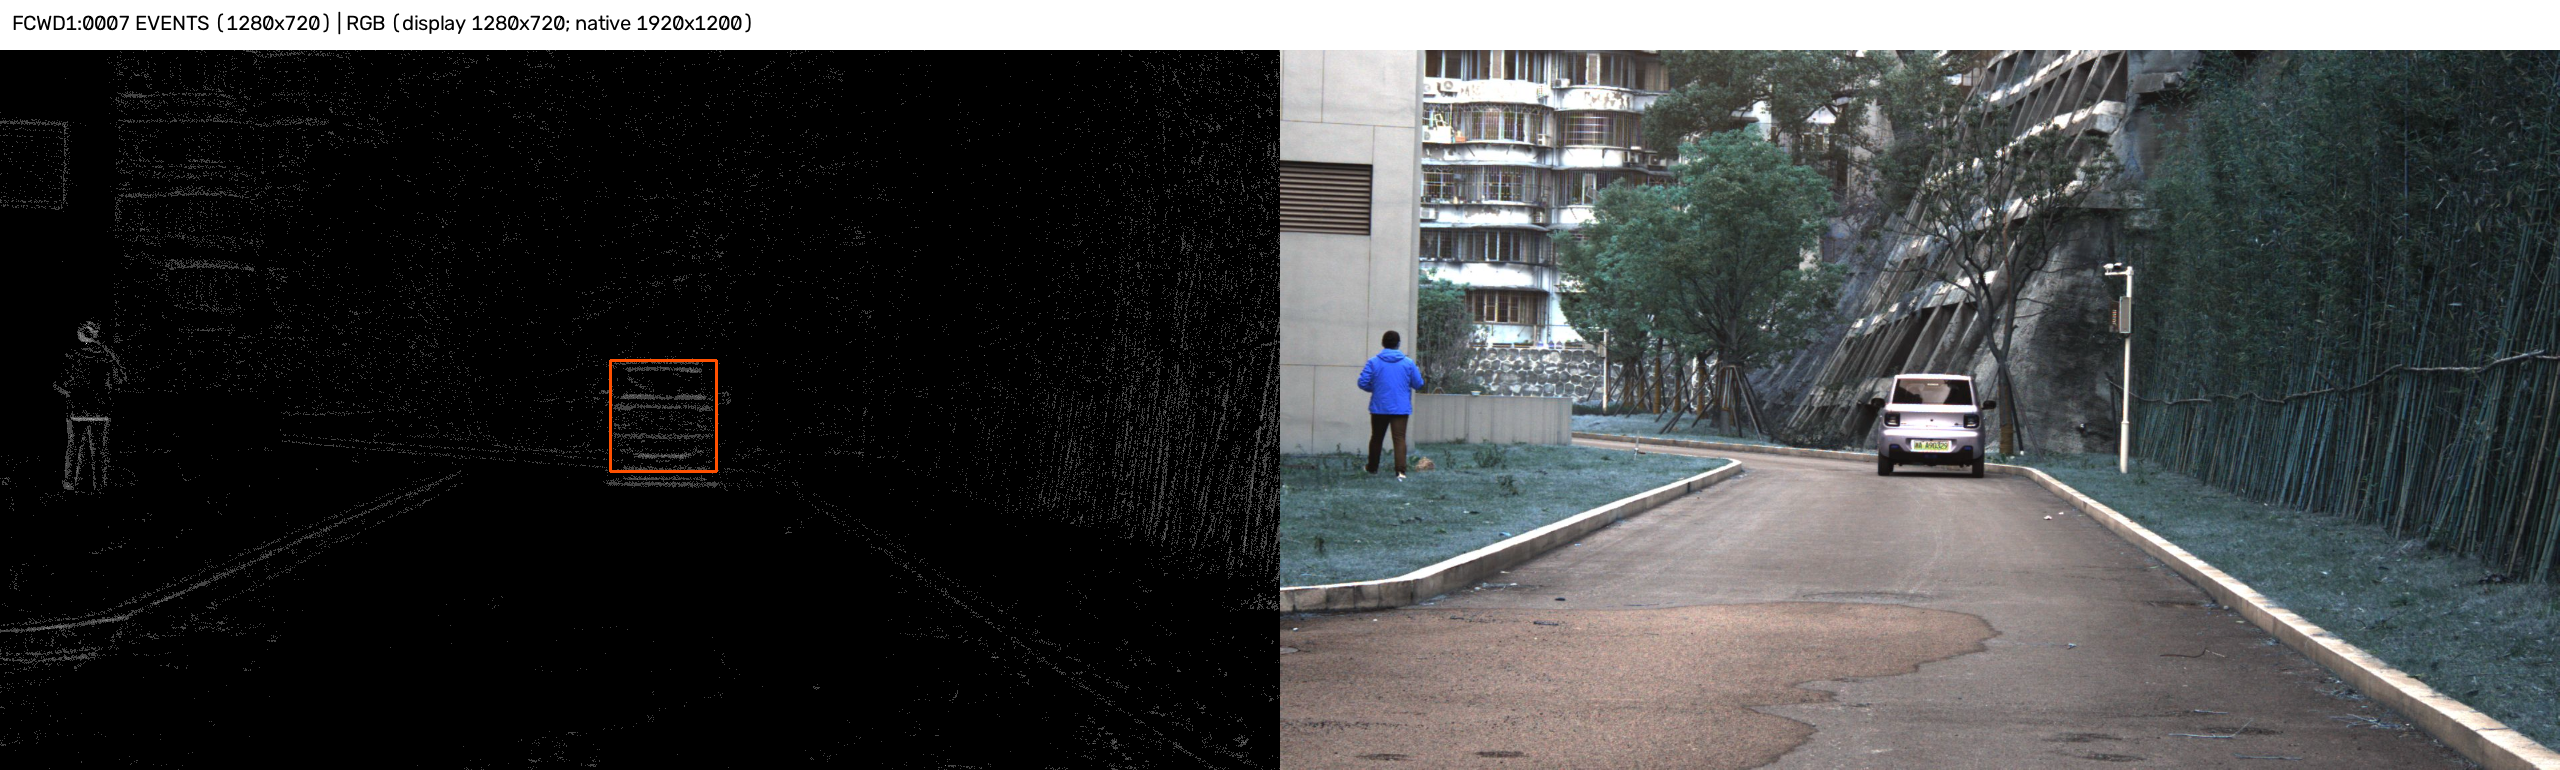
\includegraphics[width=\linewidth]{figures/fcwd_example.png}
\caption{\textbf{Event and RGB appearance for one object region.} FCWD1:0007 illustrates the cross-modal alignment problem. The orange region is the original visualization overlay.}
\label{fig:sensors}
\end{figure}

The eAP adapter reconstructs local targets from public three-dimensional tracks, whereas the benchmark uses private smoothed labels. Results therefore keep reconstructed eAP targets, EvTTC labels, and official GarlTTC labels in separate evaluation populations. \evidence{M01}

\subsection{Predictive embedding learning}
The generic JEPA implementation encodes a context representation with an online encoder $f_\theta$ and predicts a future latent conditioned on a horizon identifier:
\begin{equation}
 z_t=f_\theta(V_t),\qquad
 \widehat z_{t+h}=g_\psi(z_t,e_h),\qquad
 z_{t+h}^{\star}=\operatorname{sg}\bigl(f_\xi(V_{t+h})\bigr).
\end{equation}
The target starts from the online weights and is updated by an exponential moving average,
\begin{equation}
 \xi\leftarrow m\xi+(1-m)\theta.
\end{equation}
For multihorizon samples, a validity mask excludes unavailable future pairs from the alignment objective. The trainer supports normalized Smooth-L1 alignment, dense token prediction, spatial or tubelet masking, and variance or \texttt{visreg} regularization. Each experiment records its active loss configuration. \evidence{M04}

The V8 attribution experiment copies the \texttt{CausalScaleTTC} endpoint encoder and predicts three views of an unlabeled third endpoint from two earlier endpoints: dense features, a global geometry token, and foreground logits. Its objective is
\begin{equation}
 \mathcal L_{\mathrm{V8}}=\tfrac13\left(
 \mathcal L_{\cos}(\widehat D_2,D_2^\star)
 +\mathcal L_{\cos}(\widehat g_2,g_2^\star)
 +\mathcal L_{\mathrm{SL1}}(\widehat F_2,F_2^\star)\right).
\end{equation}
The scalar foreground-logit view uses Smooth-L1 because one-dimensional cosine similarity is almost everywhere constant. A frozen target encoder processes the future endpoint in evaluation mode under \texttt{no\_grad}. TTC, boxes, masks, category, metadata, geometry losses, contrastive losses, VICReg, and router outputs remain outside this objective. \evidence{M05}

V8 schedules EMA momentum by cosine interpolation between configured endpoints. It measures dispersion, effective rank, covariance trace, intersample similarity, and norm for the dense, global, and foreground views. A persistent-collapse rule aborts training when these diagnostics remain below their thresholds. Downstream probes then measure TTC utility.

V8 includes strict encoder transfer, random-frozen and scratch controls, partial-finetuning allowlists, and a shuffled-future control. The shuffled control uses a deterministic cross-track derangement that preserves the future marginal while holding the batch schedule, model, optimizer, update count, masking, augmentation, and EMA schedule fixed. Track identities construct the derangement and are excluded from model inputs. The declared gates require improvement over these controls before attributing a gain to predictive temporal structure. \evidence{M05}

\subsection{Spatial structure and temporal memory}
The high-resolution tubelet path preserves tokens as $[B,T,P,D]$, with distinct temporal and spatial patch axes. Images are padded on the right and bottom to a ceiling-based patch grid; invalid temporal positions and spatial padding carry masks. Windowed attention mixes spatial positions within a frame before a temporal mixer receives each patch trajectory. This separation prevents flattened raster order from being interpreted as time. \evidence{M06}

A block-causal Transformer permits attention among all spatial patches at the same instant and all earlier instants, while masking later frames. If token $i$ belongs to time $t_i$ and token $j$ to time $t_j$, its attention mask is $A_{ij}=\mathbf 1[t_j>t_i]$. A triangular token mask would impose an arbitrary left-to-right spatial ordering within each frame, so the implementation supplies the temporal block mask explicitly.

The recurrent delta-memory alternative maintains a separate matrix state per spatial patch and attention head. Writing the channelwise retention as $\alpha_t$, the implemented update is
\begin{align}
 \widetilde S_t&=\operatorname{diag}(\alpha_t)S_{t-1},\\
 e_t&=v_t-k_t^\top\widetilde S_t,\\
 S_t&=\widetilde S_t+\beta_t k_t e_t^\top,\qquad o_t=q_t^\top S_t.
\end{align}
Invalid patch steps retain the previous state and emit zero. State accumulation uses FP32, and the output returns to the input value dtype. Chunked execution passes explicit state between chunks and returns a detached final state, avoiding state shared between sequences. The causal recurrence uses no custom CUDA kernel. Tests establish equivalence between chunked and unchunked computation; runtime experiments determine deployment speed. \evidence{M06}

Before allocation, the implementation estimates quadratic attention-score memory,
$B H (TP)^2 b$ bytes for $H$ heads and $b$ bytes per value, and rejects layouts above the configured safety limit. Runtime evaluation reports observed memory, preprocessing time, and throughput.

\subsection{Causal scale, local transport, and TTC anchors}
The geometry-constrained model learns a foreground probability field and differentiable visible extent for each endpoint. It forms geometry tokens from the encoder token, log-height, centroid, foreground fraction, and sensor support. The analytic log-scale difference is supplemented by a bounded residual,
\begin{equation}
 r=\log h_2-\log h_1+\delta(a,b),\qquad
 \delta(a,b)=r_{\max}\tanh\!\left(\frac{u(a,b)-u(b,a)}2\right).
\end{equation}
With deterministic evaluation and reversed transport inputs, the residual changes sign under endpoint reversal. The primary output remains geometry-bound; the auxiliary direct inverse-TTC head does not feed into it. \evidence{M07}

The timestamp anchor matters. Under constant relative speed and apparent size inversely proportional to distance, the \emph{current-endpoint} inverse TTC is
\begin{equation}
 q_2=\frac{e^r-1}{\Delta t},\qquad T_2=\frac{\Delta t}{e^r-1}.
\label{eq:current-anchor}
\end{equation}
The learned-height-ratio reference implements
\begin{equation}
 T_1=\frac{\Delta t}{1-h_1/h_2}
     =\frac{\Delta t}{1-e^{-r}}=T_2+\Delta t,
\label{eq:start-anchor}
\end{equation}
which is anchored at the earlier endpoint under the same assumptions. Each route uses the convention determined by its label timestamp and evaluator. The benchmark phase defined below is a metric coordinate distinct from the current-endpoint log-scale difference. \evidence{M07,M10}

The transport extension derives event-native motion evidence from dense features $D_1,D_2$. It builds cosine correlations in a local neighbourhood $\mathcal N(p)$ and obtains expected displacement by
\begin{equation}
 P(\delta\mid p)=\frac{\exp\!\left(\langle\bar D_1(p),\bar D_2(p+\delta)\rangle/\tau\right)}
 {\sum_{\delta'\in\mathcal N(p)}\exp\!\left(\langle\bar D_1(p),\bar D_2(p+\delta')\rangle/\tau\right)},
 \quad d(p)=\sum_{\delta\in\mathcal N(p)}P(\delta\mid p)\delta.
\end{equation}
Out-of-bounds candidates are masked before softmax. The resulting summaries include translation, anisotropic and isotropic divergence, flow magnitude, confidence margin, entropy, and forward--reverse cycle error, with additional foreground-weighted variants. Coarse-to-fine models mix measurements from two scales through a learned gate. Shifted views replace a $[B,C,K,H,W]$ unfolded tensor to reduce intermediate memory. \evidence{M08}

Training-time RGB distillation introduces privileged visual supervision. The A4 DINOv3 teacher \citep{dinov3} supplies local cosine-similarity maps at six fixed feature-grid offsets. An L1 loss transfers these spatial relationships without requiring equal channel dimensions; slicing avoids circular wraparound. The student consumes events alone at inference, making this route privileged distillation rather than label-free self-supervision. \evidence{M09}

\subsection{Phase-domain routing and temporal refinement}
\label{sec:phase-refinement}
The later benchmark coordinate is
\begin{equation}
 \phi(T)=-\log\left(1-\frac{d}{T}\right),\qquad d=0.1\ \mathrm{s},
 \quad T<0\ \text{or}\ T>d.
\label{eq:benchmark-phase}
\end{equation}
Its inverse uses $q=-\operatorname{expm1}(-\phi)/d$. The implementation clamps phase to its configured support and saturates TTC magnitude at $60$ seconds; zero phase maps to $+60$ seconds. Saturation defines finite numerical output, while signed negative values represent recession. \evidence{M10}

\begin{figure}[H]
\centering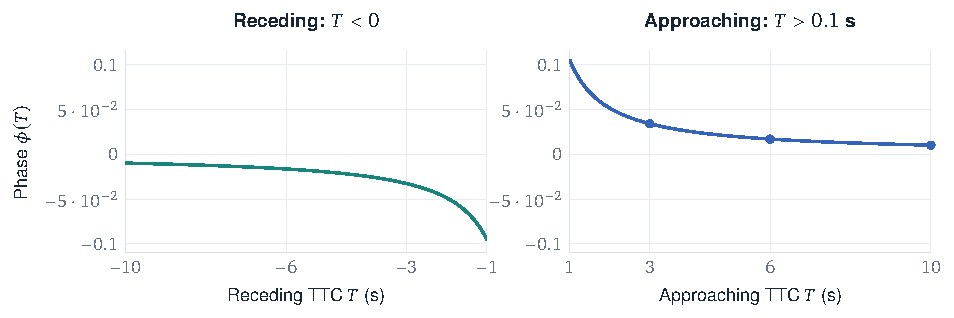
\includegraphics[width=\linewidth]{figures/rev_phase.pdf}
\caption{\textbf{Signed phase geometry.} Analytical curves show $|T|\in[1,10]$\,s on common vertical scales, with approaching-band markers at 3, 6, and 10\,s. The zoom excludes $[0,0.1]$\,s and the adjacent singularities.}
\label{fig:phase-geometry}
\end{figure}

The Simplex risk router selects among frozen expert TTCs by predicting relative expected absolute-phase costs. For three sorted expert phases, convexity and the 1-Lipschitz property of $\mathbb E|a-Y|$ imply ordered secant slopes $-1\leq s_0\leq s_1\leq1$. Softmax increments parameterize these constraints; integrating the slopes across expert-phase gaps yields relative costs. Hard selection returns one original expert prediction under a fixed tie order. The learned quantities are relative selection costs rather than calibrated collision probabilities. \evidence{M11}

The temporal refiner predicts a correction from a bounded feature history and four timing channels using a masked two-layer GRU; a causal Transformer provides the matched control. Histories require a contiguous valid suffix, and missing prefixes leave recurrent state unchanged. Residual mode anchors the phase at the median of the \emph{current} experts,
\begin{equation}
 \widehat\phi=\operatorname{median}(\phi_1,\phi_2,\phi_3)+0.03\,a_\theta(H).
\end{equation}
Separate heads predict phase-quantile widths and relative costs for the original experts; the latter do not estimate risk for the corrected output. Training combines phase absolute error, pinball losses, and relative-cost regression. Globally defined query mass supplies the weights without minibatch renormalization. Sparse-history variants retain selected slots from a longer history and recompute timing gaps from integer anchors, preserving cold starts and the original query population. \evidence{M12}

\subsection{Multimodal complement and uncertainty boundaries}
The later joint-measurement complement anchors on RGB phase and learns a correction from RGB features, event features, and the RGB phase itself:
\begin{equation}
 \widehat\phi=\phi_{\mathrm{RGB}}+s\,g_\theta
   ([z_{\mathrm{RGB}},z_{\mathrm{event}},\phi_{\mathrm{RGB}}]).
\end{equation}
The final layer starts at zero, so the initial prediction reproduces the RGB anchor up to native phase conversion. A matched ZERO control removes the complete event-feature block, including admitted event-clock features, while retaining network capacity. When RGB is absent, the model copies the event TTC without applying correction or averaging. The paired TRUE--ZERO comparison isolates the contribution of event information to the learned RGB correction. \evidence{M13}

Uncertainty has multiple meanings across these families. The causal-scale route predicts log-variance in log-ratio space and propagates it through the local Jacobian. For $q=\operatorname{expm1}(r)/\Delta t$,
\begin{equation}
 \operatorname{Var}(q)\approx \frac{e^{2r}}{\Delta t^2}\operatorname{Var}(r),\qquad
 \operatorname{Var}(T)\approx \frac{\Delta t^2e^{2r}}{(e^r-1)^4}\operatorname{Var}(r).
\end{equation}
The singularity near zero expansion requires separate finite-output and \texttt{known} indicators. The implementation marks unsupported or near-zero log-ratio predictions unknown and derives model-based threshold probabilities from an inverse-TTC Gaussian approximation. Empirical calibration requires measurements of coverage, calibration error, and corruption response. The temporal refiner's phase quantiles carry a different meaning from collision-class probabilities. \evidence{M07,M12}

\subsection{Optimization and execution semantics}
Component losses keep their true counts over each effective batch, and tail top-$k$ selection uses the complete effective batch instead of separate microbatches. Activation recomputation preserves random-number-generator state, keeping gradient accumulation and recomputation equivalent to the stated objective. The joint-measurement loss includes teacher relations, unlike the label-free JEPA loss. \evidence{M14}

Deployment optimizations include bounded event history, chunked memory, persistent input state, reusable feature caches, and graph execution. Because each changes state lifetime, numerical-parity tests accompany every admitted path. Runtime measurements state the associated preprocessing and inference boundary.
